\documentclass[a4paper,12pt]{article}
\usepackage[utf8]{inputenc}
\usepackage{amsmath}
\usepackage{graphicx}
\usepackage{booktabs}
\usepackage{subfigure}
\usepackage{subcaption}
\usepackage{float}
\usepackage{url}
\graphicspath{ {./images/} }


\title{\textbf{Análise de casos de Dengue no Brasil: impactos, sintomas e a influência dos casos na Pandemia da COVID-19}}

\author{
    \normalsize
    \textbf{Alex Júnio Maia de Oliveira (aluno)} \\ 
    \normalsize
    \textbf{Bruno Ferreira  Salvi (aluno)} \\
    \normalsize
    \textbf{João Pedro Jerônimo de Oliveira (aluno)} \\
    \normalsize
    \textbf{Matheus Vilarino de Sousa Pinto (aluno)} \\
    \normalsize
    \textbf{Thalis Ambrosim Falqueto (aluno)} \\
    \normalsize
    \textbf{Orientador: Rafael de Pinho André} \\
    \normalsize
    \ Fundação Getúlio Vargas - FGV \\
    \normalsize
    \ Graduação em Ciência de Dados e Inteligência Artificial
}
\date {\today}

\begin{document}

\maketitle

\noindent\textbf{RESUMO} \\ \\O artigo tem como objetivo geral o estudo de um conjunto de dados disponibilizado pelo SINAN (Sistema de Informação de Agravos de Notificação) relacionados a uma coleta feita pelo Sistema Único de Saúde, referente a dengue no Brasil nos anos de 2021 a 2024. A metodologia inclui o pré-processamento, a análise exploratória dos dados e o testes das hipóteses, validando ou as invalidando.  Além disso, busca-se identificar padrões, correlações e observações relevantes por meio de estatística descritiva e visualização de dados feitas usando as principais ferramentas ensinadas no curso nativas do \emph{Python}, como \emph{pandas} e \emph{numpy}, além de ferramentas de plotagem como \emph{matplotlib}, \emph{seaborn} e \emph{streamlit}. Por fim, o controle de versionamento foi realizado por meio de \emph{git} e \emph{git-flow}, proporcionando um melhor gerenciamento, organização e estruturação do estudo.

\vspace{0.5cm}

\noindent\textbf{Palavras-chave}: Dengue; Python; análise de dados

\section{Introdução}
O trabalho propõe a escolha de um dataset, a partir do qual devem ser feitos o levantamento de perguntas e hipóteses sobre a base de dados. Após uma análise criteriosa de diversas fontes de dados, foi selecionado o dataset disponibilizado pelo Sistema de Informação de Agravos de Notificação (SINAN)\footnote{Pode ser encontrado em: \url{https://www.kaggle.com/datasets/henriquerezermosqur/dados-sus-sinan-dengue-2021-2024}}, referente aos casos de dengue. Com base nesse conjunto de dados, foram formuladas cinco hipóteses principais para guiar o estudo e permitir a exploração de padrões e considerações relevantes:

\begin{itemize}
    \item Quais são os conjuntos de sintomas principais que levaram ao óbito/internação?
    \item Casos de dengue seguem uma distribuição normal com relação à data do início dos sintomas (ou seja, tem alguma relação com temperatura ou estação)? Qual a distribuição dos casos totais e a proporção de mortes por dengue em cada unidade da federação?
    \item Existe alguma relação entre os exames e os sintomas (por exemplo, há tendência de se fazer exame X dependendo dos sintomas)? 
    \item Pessoas em ocupações relacionadas à zona rural contrairam dengue em seu trabalho?
    \item Nos períodos de Covid-19, houve alguma mudança em relação à quantidade de pessoas diagnosticadas com dengue? Além disso, nesses períodos, o tempo de demora entre a entrada no hospital e a hora do exame aumentou?
\end{itemize}

Com base nas hipóteses propostas, a próxima etapa consiste na verificação por meio de uma análise crítica e detalhada dos dados. Essa abordagem visa garantir a precisão dos resultados e a solidez das interpretações, possibilitando uma compreensão aprofundada dos padrões e dinâmicas dos casos de dengue no Brasil. Especial atenção será dada às variações observadas durante o contexto pandêmico da COVID-19, bem como às áreas rurais, que apresentam características epidemiológicas distintas.

\clearpage

\section{Metodologia}
O grupo optou por utilizar uma base de dados disponibilizado pelo SINAN que abrange casos de dengue em todo o território brasileiro. As análises foram realizadas na lingugaem de programação \emph{Python}, manuseando bibliotecas externas como Numpy, Pandas, Seaborn, Matplotlib e Geopandas, além de bibliotecas \emph{built-in} como os e sys.

Para conduzir a análise exploratória dos dados coletados, foram aplicados conceitos de estatistíca descritiva\footnote{BUSSAB, Wilton de Oliveira; MORETTIN, Pedro Alberto. Estatística básica. 9. ed. São Paulo: Saraiva, 2017} tais como coeficiente de contingência, correlação e covariância, permitindo uma melhor compreensão das relações entre as variáveis envolvidas.

Dessa forma, a partir de tais análises, as hipóteses seriam validadas ou refutadas, auxiliando assim no aprofundadmento do estudo das causalidades da dengue em espaço brasileiro.


\section{Objetivos}

O estudo tem como objetivos analisar os casos de dengue e compreender sua distribuição geral no cenário brasileiro, averiguar a sua correlação com o período pandêmico e fomentar a pesquisa no âmbito da prevenção da doença, ambrangendo tecnologias, análises de dados e identificação de padrões para a melhora do bem-estar da população brasileira e, por conseguinte, as populações afetadas pela enfermidade.

Espera-se que este estudo contribua de forma significativa para o avanço do conhecimento científico sobre a dengue, fornecendo abordagens relevantes para a formulação de políticas públicas mais eficazes e para o aprimoramento das estratégias de controle e prevenção da doença.

\section{Desenvolvimento}

Como parte principal do artigo, o desenvolvimento enfatizará a legitimação das teorias propostas na introdução, buscando um entendimento completo da base de dados escolhida.

\subsection{Hipótese 1}
\emph{"Quais são os conjuntos de sintomas que mais levam à internação ou óbito do paciente?"}

Sabe-se que a dengue é uma doença caracterizada por uma ampla gama de sintomas e, dessa maneira, seria natural se questionar qual seria o conjunto de sintomas mais associado à piora do estado de saúde dos pacientes.
Foram levados em conta vários sintomas, sendo os principais deles :
\begin{itemize}
    - Febre Alta : reação de defesa do organismo, caracterizada pela elevação da temperatura corporal entre 39 a 40 graus celsius;\\
    - Mialgia : Dores musculares intensas; \\
    - Dor de Cabeça : Dor intensa na região frontal;\\
    - Hipertensão : niveis elevados de pressão arterial;\\ 
    - Naúsea : enjôo seguido de fraqueza e falta de apetite;\\
    - Vômito : quadros de vômitos persistentes e dores aabdominais;\\
    - Renal : prejudicação do sistema renal do indivíduo.\\
\end{itemize}

O cerne da questão está na forma de analizar os dados disponíveis: "como realizá-la?". Para respondê-la, podemos então olhar para os pacientes que obtiverem como resultado final o óbito e achar a razão óbito/ocorrência para cada sintoma. 

Aqui está a tabela dos sintomas ordenada pela razão de óbito:

\begin{table}[H]
    \centering
    \caption{Dados de Sintomas e Razão de Óbito - Parte 1}
    \begin{tabular}{@{}lccc@{}}
        \toprule
        \textbf{Conjunto de Sintomas} & \textbf{Óbitos} & \textbf{Ocorrências} & \textbf{Razão \%} \\ 
        \midrule
        Renal & 61 & 668 & 9.13 \\
        Hematológico & 41 & 515 & 7.96 \\
        Hipertensão & 485 & 7669 & 6.32 \\
        Hepatopatia & 19 & 403 & 4.71 \\
        Vômito & 448 & 13493 & 3.32 \\
        Dor nas Costas & 232 & 6891 & 3.37 \\
        Petequias & 97 & 3224 & 3.01 \\
        Náusea & 462 & 16249 & 2.84 \\
        Leucopenia & 157 & 5563 & 2.82 \\
        Mialgia & 728 & 26346 & 2.76 \\
        Artralgia & 146 & 5356 & 2.73 \\
        Febre & 773 & 28933 & 2.67 \\
        Cefaleia & 539 & 22860 & 2.36 \\
        Dor Retro & 174 & 7696 & 2.26 \\
        Conjuntivite & 23 & 1009 & 2.28 \\
        Exantema & 89 & 4143 & 2.15 \\
        Artrite & 68 & 2026 & 3.36 \\ 
        \bottomrule
    \end{tabular}
    \label{tab:symptom_data_1}
\end{table}

\begin{table}[H]
    \centering
    \caption{Dados de Sintomas e Razão de Óbito - Parte 2}
    \begin{tabular}{@{}lccc@{}}
        \toprule
        \textbf{Conjunto de Sintomas} & \textbf{Óbitos} & \textbf{Ocorrências} & \textbf{Razão \%} \\ 
        \midrule
        Conjuntivite | Hematológico & 7 & 46 & 15.22 \\
        Dor nas Costas | Hematológico & 17 & 117 & 14.53 \\
        Artralgia | Hematológico & 16 & 108 & 14.81 \\
        Dor nas Costas | Renal & 19 & 169 & 11.24 \\
        Renal | Hipertensão & 45 & 417 & 10.79 \\
        Vômito | Renal & 28 & 273 & 10.26 \\
        Exantema | Renal & 7 & 70 & 10.00 \\
        Petequias | Renal & 6 & 61 & 9.84 \\
        Vômito | Hematológico & 20 & 209 & 9.57 \\
        Cefaleia | Hematológico & 31 & 329 & 9.42 \\
        Febre | Renal & 48 & 517 & 9.28 \\
        Artrite | Renal & 6 & 64 & 9.38 \\
        Mialgia | Renal & 44 & 483 & 9.11 \\
        Cefaleia | Renal & 33 & 363 & 9.09 \\
        Conjuntivite | Hepatopatia & 3 & 34 & 8.82 \\
        Dor Retro | Renal & 12 & 137 & 8.76 \\
        Febre | Hematológico & 39 & 447 & 8.72 \\
        Petequias | Hepatopatia & 5 & 62 & 8.06 \\
        Mialgia | Hematológico & 30 & 379 & 7.92 \\
        Náusea | Renal & 27 & 345 & 7.83 \\
        Hematológico | Hipertensão & 14 & 185 & 7.57 \\
        Náusea | Hematológico & 19 & 259 & 7.34 \\
        Artralgia | Renal & 8 & 110 & 7.27 \\
        \bottomrule
    \end{tabular}
    \label{tab:symptom_data_2}
\end{table}



Percebe-se que o número de óbitos não indica uma alta mortalidade (coluna razão), pois um sintoma mortal pode ser mais raro do que um com efeitos mais amenos. Logo, ao realizar a análise da última coluna, podemos notar que os sintômas renais, hematológicos e hipertensão possuem uma alta taxa de mortalidade quando comparados com os outros sintomas individualmente. Já quando tomamos conjuntos dois a dois, conjuntivite e hematológicos acabam ficando em primeiro lugar.

Notamos que os sintomas de febre, mialgia e cefaleia são os que mais aparecem em indivíduos que sofreram a hospitalização. Logo, apesar de terem uma alta incidência nos infectados, não parecem agravar tanto a situação deles.

Os resultados obtidos desta parte podem ser usados para avaliar a urgência de tratamento de um paciente com base em seus sintomas. 



\subsection{Hipótese 2}
\emph{"Casos de dengue seguem uma distribuição normal com relação a data do início dos sintomas (ou seja, tem alguma relação com temperatura ou estação)? Qual a distribuição do total de casos e da taxa de mortalidade por estado?"}

\\\\\
Conhecer as distribuições dos casos totais de dengue por ano divididos por mês é de suma importância para a compreensão do estudo, pois dessa forma temos uma noção geral dos períodos de maior volume dos casos de dengue.

Além disso, é intrínseco conhecer quais regiões brasileiras sofrem com voluptuosas ocorrências da doença e quais têm uma maior proporção de óbitos.

Para analisar os dados de todos os anos (2021 a 2024) com relação à data do início dos sintomas de cada caso relatado na base principal, pode-se realizar uma exibição de um histograma juntamente com sua linha de distribuição (\emph{kdeplot}).

Ao fazer tais gráficos, tem-se como resultado:

\begin{figure}[H]
    \centering
    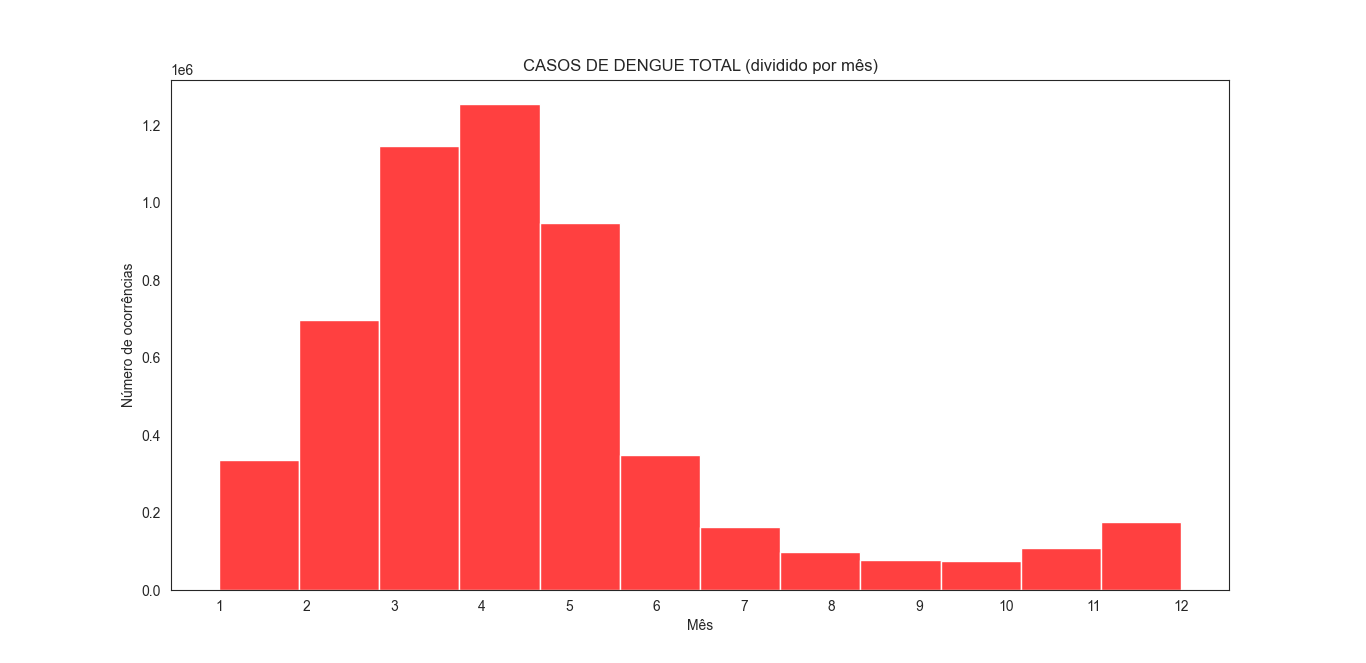
\includegraphics[width=1.0\textwidth]{images/By month total.png}
    \caption{Casos de dengue 2021-2024 (divido por mês)}
    \label{fig:by_month_total}
\end{figure}

\begin{figure}[H]
    \centering
    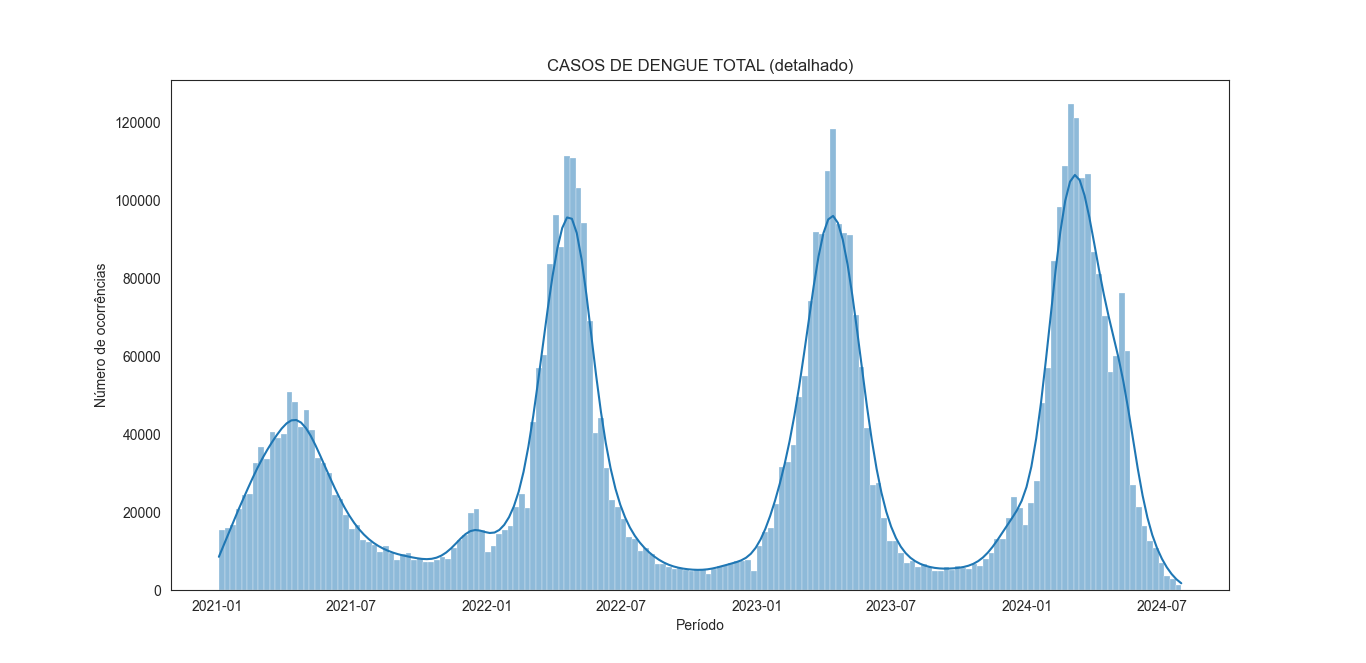
\includegraphics[width=1.0\textwidth]{images/By period (detailed) total.png}
    \caption{Casos de dengue 2021-2024 (divido por período)}
    \label{fig:by_period_total}
\end{figure}

Portanto, observa-se que no período de março (mês 3) a maio (mês 5), tem-se um pico no número de casos de dengue. Isso deve-se pois neste período há um aumento nas temperaturas médias e se inicia um período de alta pluviosidade, condições essas que atraem o mosquito da dengue (\emph{Aeds aegypti}).

Ademais, realizando a divisão dos casos totais de dengue e a proporção de mortes em cada unidade da federação, tem-se o seguinte:

\begin{figure}[H]
    \centering
    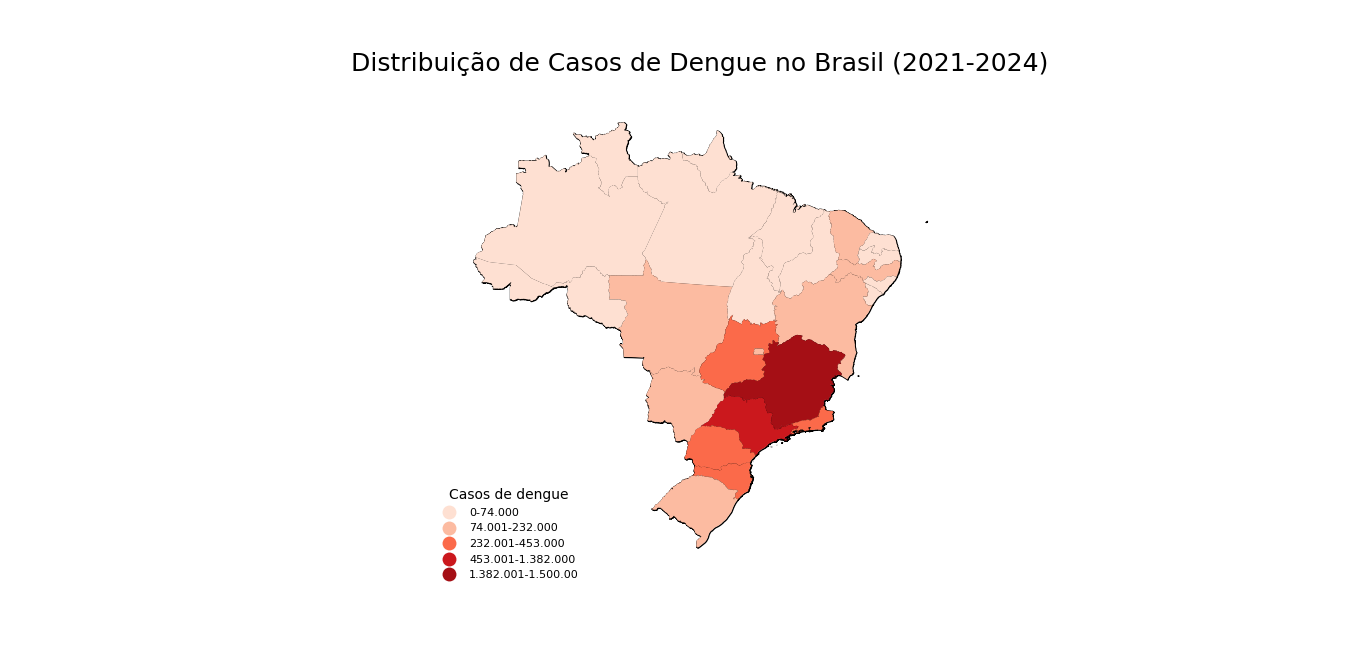
\includegraphics[width=1.0\textwidth]{images/Heatamp (uf) total.png}
    \caption{Casos de dengue 2021-2024 (divido por estado)}
    \label{fig:heatmap_total}
\end{figure}

\begin{figure}[H]
    \centering
    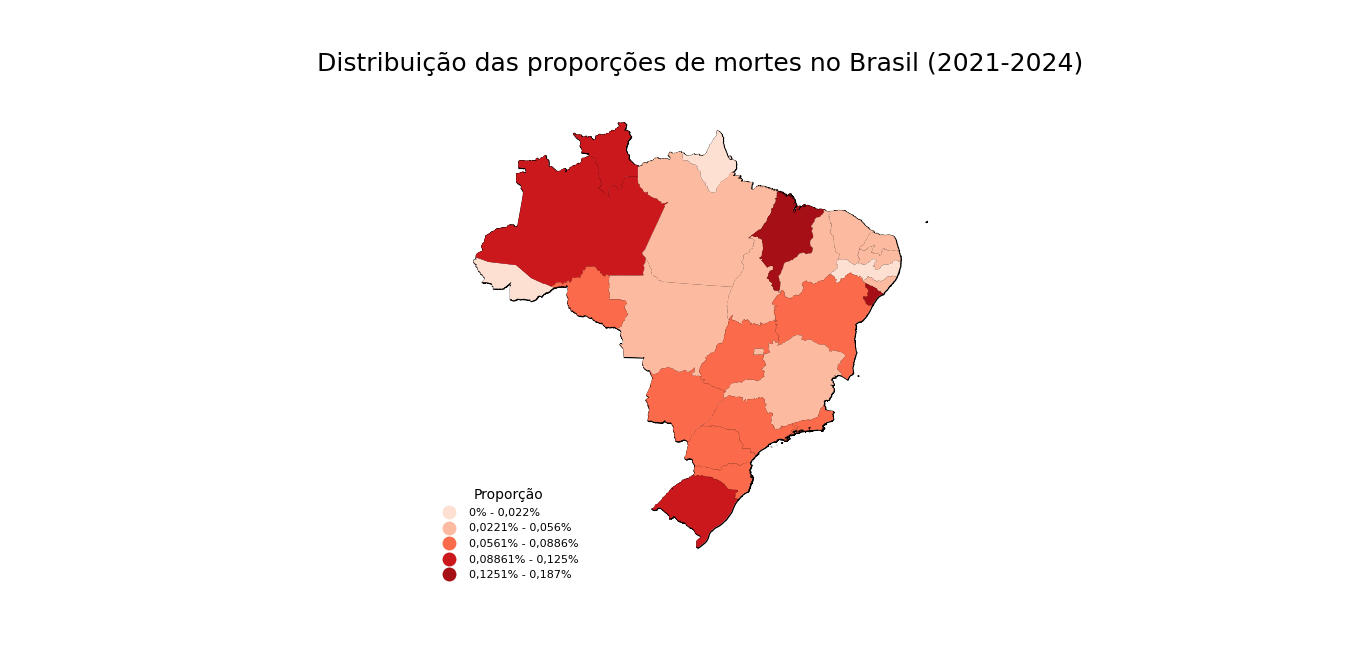
\includegraphics[width=1.0\textwidth]{images/Heatmap (uf) proportion.png}
    \caption{Taxa de mortalidade 2021-2024 (divido por estado,)}
    \label{fig:heatmap_proportion}
\end{figure}

Logo, a região Sudeste do Brasil sofre com um maior número de casos de dengue. No entanto, observando a proporção dos óbitos por cada estado, Amazonas, Rio Grande do Sul, Roraima, Maranhão e Alagoas têm taxas de mortalidade alarmantes.

Essas disparidades podem ser atribuídas a uma combinação de fatores, como a qualidade do sistema de saúde, a disponibilidade de recursos para o tratamento da doença e as condições socioeconômicas das populações afetadas. A análise dessas proporções é importante para entender não apenas a epidemiologia da dengue, mas também para identificar as partições que necessitam de intervenções imediatas para mitigar a mortalidade e aprimorar a resposta ao surto da doença.

    
\subsection{Hipótese 3}
\emph{"Existe alguma relação entre os exames e os sintomas? (Como por exemplo, há tendência de se fazer exame X dependendo dos sintomas?)"}

É notória a relevância dos exames para a classificação do tipo e tratamento da dengue, além disso, os possíveis sintomas que um enfermo pode possuir são variados. A partir disto, pode-se ter um questionamento natural acerca da relação entre ambas as variáveis, o que poderia indicar uma \textbf{tendência para um exame X} dependendo do \textbf{sintoma do paciente}.

Para verificar se existe tal grau de correlação entre os exames e os variados sintomas, devemos calcular o coeficiente de contingência\footnote{BUSSAB, Wilton de Oliveira; MORETTIN, Pedro Alberto. \textit{Estatística básica}. 9. ed. São Paulo: Saraiva, 2017, p. 76-79.}
 entre as variáveis (levando em conta a análise entre qualitativa e qualitativa). 

\begin{table}[H]
    \centering
    \caption{Relação de cada sintoma com cada tipo de exame (coeficiente de contingência)}
    \begin{tabular}{lcccc}
        \toprule
        & VIRAL & NS1 & PCR & SORO \\ \midrule
        FEBRE & 0.008843341 & 0.07073418 & 0.032843042 & 0.08271805 \\
        MIALGIA & 0.0042822515 & 0.08398538 & 0.014000116 & 0.07025483 \\
        CEFALEIA & 0.005272286 & 0.07877089 & 0.014883856 & 0.056865178 \\
        EXANTEMA & 0.0042484426 & 0.05956145 & 0.016023878 & 0.076502524 \\
        VOMITO & 0.004277692 & 0.034537956 & 0.012604693 & 0.018651566 \\
        NAUSEA & 0.0070605674 & 0.044488683 & 0.021723958 & 0.026098222 \\
        DOR\_COSTAS & 0.009681542 & 0.0509112 & 0.018726623 & 0.03377638 \\
        CONJUNTVIT & 0.0022646226 & 0.035315834 & 0.0046890657 & 0.014131442 \\
        ARTRITE & 0.0026269057 & 0.058515746 & 0.0067389817 & 0.02034513 \\
        ARTRALGIA & 0.010431411 & 0.09557537 & 0.008657125 & 0.027218288 \\
        PETEQUIA\_N & 0.0052888487 & 0.040161483 & 0.012530279 & 0.072297454 \\
        LEUCOPENIA & 0.0022609849 & 0.03913427 & 0.014333641 & 0.02951866 \\
        DOR\_RETRO & 0.007177497 & 0.086504884 & 0.013840019 & 0.03679464 \\
        DIABETES & 0.0048826593 & 0.0025543477 & 0.012184973 & 0.029313331 \\
        HEMATOLOG & 0.010838465 & 0.004643966 & 0.009706085 & 0.0127382595 \\
        HEPATOPAT & 0.006810185 & 0.0037634424 & 0.0077766073 & 0.013733226 \\
        RENAL & 0.007903093 & 0.005708144 & 0.0077094375 & 0.013379313 \\
        HIPERTENSA & 0.0052119107 & 0.014869342 & 0.021061204 & 0.041687407 \\
        ACIDO\_PEPT & 0.011652101 & 0.006113838 & 0.008748848 & 0.010554269 \\
        AUTO\_IMUNE & 0.0052067423 & 0.0035075748 & 0.0066045304 & 0.009411497 \\
        \bottomrule
    \end{tabular}
    \label{tab:sintomas_resultados}
\end{table}

Portanto, de acordo com a tabela apresentada, pode-se observar que os coeficientes de contingência entre a maioria dos sintomas e dos exames são muito pequenos, ou seja, tem-se um grau mínimo de relação entre ambas variáveis.


\subsection{Hipótese 4}
\emph{"Pessoas em ocupações relacionadas a zona rural pegaram a dengue em seu trabalho?"}

Tendo em vista a existência de uma coluna que registra a ocupação de cada paciente no dataframe principal, realizou-se uma análise que visava procurar indícios sobre o trabalho que cada indivíduo realizava e sua possível contração de dengue. 

Uma das lógicas indagações é supor que pessoas que trabalham no meio rural possuem maior chance de contraírem a dengue, pois suas ocupações estão mais predispostas a exposição ao ar livre, maior presença de criadouros e consequentemente água parada, menos infraestrutura e saneamento, além de menos controle sobre os vetores de propagação da doença.

Por essa ótica, seria interessante estabelecer uma relação entre a coluna de ocupação e a coluna que registra se o paciente adquiriu a doença em decorrência das condições/situação de trabalho, infelizmente, a interseção de valores válidos em ambas as colunas é nula e por isso, essa análise não poderá ser feita.

Entretando, pode-se analisar a frequência que ocupações relacionadas ao meio rural aparecem no dataset e compará-las com outras ocupações gerais. Com este fim, foi feito um estudo seguindo estes passos: 
-  Obteve-se um dataset secundário retirado do site da CBO, Classificação Brasileira de Ocupações, que consta a relação do código contido no dataset principal e a descrição do seu título relacionando códigos em comum, pode-se filtrar por ocupações que contiam termos relacionados ao meio rural, como "agro", "pecuária" e "rural", para uma análise mais fidedigna, foram removidos cargos com alcunhas "gerente", "economista", "diretor" e outros, pois, em hipótese, essas funções não possuem as mesmas predisposições comuns dos outros e portanto não devem entrar nas observações. 
- Segmentando em dois conjuntos de dados, ocupações gerais e outros, realizamos cálculos para chegar na média de proporções de cada tipo de ocupação. Considerando a amostra que varia de 01/2021 até 07/2024, chegamos que a proporção das ocupações rurais é de aproximadamente 5 vezes maior que uma ocupação comum. 

Após as análises feitas acima, evidencia-se um indício que o trabalho de cada indivíduo influencia na sua chance de contrair a dengue.

\begin{figure}[H]
    \centering
    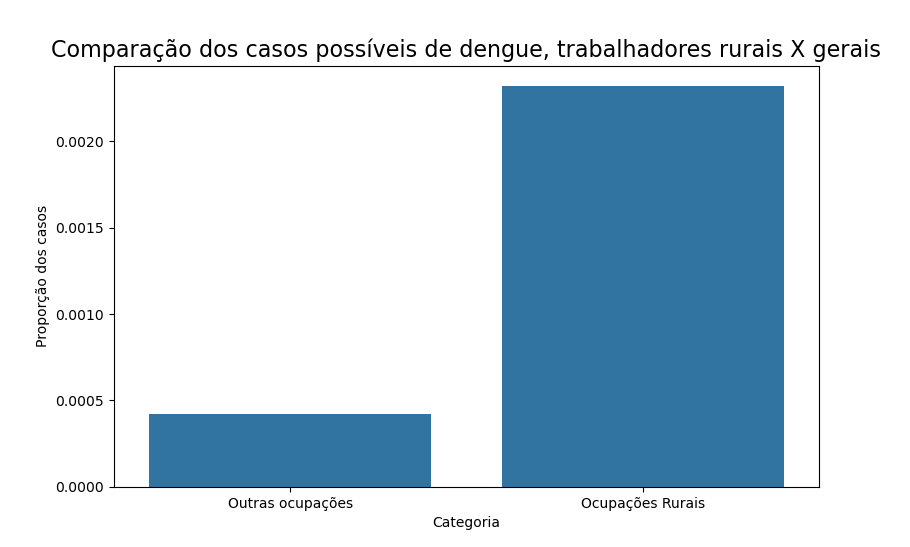
\includegraphics[width=1.0\textwidth]{images/plot_hp4.png}
    \caption{Proporção dos casos por tipo de ocupação}
    \label{fig:occupation}
\end{figure}

    
\subsection{Hipótese 5}
\emph{"Nos períodos de covid, houve alguma mudança em relação à quantidade de pessoas diagnosticadas com dengue? Além disso, nesses períodos, o tempo de demora entre a entrada no hospital e a hora do exame aumentou?
"}

Baseando-se no dataset no período coincidente com a pandemia de COVID-19, foram realizadas análises estatísticas básicas, incluindo o cálculo de quartis, desvio-padrão, média, entre outros, com o objetivo de comparar esses dados com o período pós-pandêmico. O propósito central dessas análises foi verificar a existência de uma possível relação entre o período pandêmico e um atraso no encerramento de casos de dengue, o que poderia sugerir que a pandemia do COVID-19 influenciou negativamente o controle e a gestão de outras doenças, como a dengue.

Com esse propósito, foi calculada a tabela que relaciona ambos os períodos em questão:


\begin{table}[H]
\centering
\caption{Comparação da diferença de dias entre a notificação da ocorrência até o encerramento do caso entre períodos }
\begin{tabular}{@{}l S[table-format=4.2] S[table-format=4.2]@{}}
\toprule
\textbf{Métrica}          & \textbf{01/01/21 - 30/11/22} & \textbf{30/11/22 - 31/07/24} \\ \midrule
Desvio Padrão                                 & 31.94              & 34.45              \\
Mediana (dias)            & 27.00              & 22.00              \\
1º Quartil (q1)           & 8.00               & 8.00               \\
3º Quartil (q3)           & 61.00              & 53.00              \\
Valor Mínimo (dias)       & 0.00               & 0.00               \\
Valor Máximo (dias)       & 505.00             & 545.00             \\
Total de Registros        & 2,987,188          & 2,356,590          \\
Soma dos Dias             & 102,288,377        & 75,412,113         \\
Média de Dias             & 34.24              & 32.00              \\ \bottomrule
\end{tabular}
\label{tab:comparison}
\end{table} \\

Após a análise das métricas calculadas, fica claro que o aumento repentino dos casos de Covid-19 não influência diretamente o gerenciamento dos casos de dengue, pois a mensuração entre os dois períodos não resultou numa variação significante de resultado, tome como exemplo os quartis, que apresentam uma diferença baixa, quando o apresentam.

Por outro lado, poderíamos supor uma relação entre o aumento do intervalo de tempo entre a notificação dos casos e a realização dos exames, o que poderia indicar uma correlação entre a pandemia de COVID-19 e o atraso na condução de exames de outras doenças. 

De forma análoga a anterior, foi realizado o cálculo das principais métricas dos períodos em pauta:

\begin{table}[H]
\centering
\caption{Comparação da diferença de dias entre a notificação da ocorrência até a realização do exame de dengue entre períodos}
\begin{tabular}{@{}l S[table-format=3.2] S[table-format=3.2]@{}}
\toprule
\textbf{Métrica}          & \textbf{01/01/21 - 30/11/22} & \textbf{30/11/22 - 31/07/24} \\ \midrule
Desvio Padrão  & 31.64              & 28.46              \\
Mediana (dias)            & 12.00              & 12.00              \\
1º Quartil (q1)           & 4.00               & 4.00               \\
3º Quartil (q3)           & 30.00              & 37.00              \\
Valor Mínimo (dias)       & 0.00               & 0.00               \\
Valor Máximo (dias)       & 545.00             & 465.00             \\
Total de Registros        & 646,233            & 886,315            \\
Soma dos Dias             & 14,496,361         & 20,920,025         \\
Média de Dias             & 22.43              & 23.60              \\ \bottomrule
\end{tabular}
\label{tab:comparison}
\end{table} 

A seguir da aferição dos dados, constata-se que, semelhante a tabela anterior, as diferenças das medidas calculadas não significam uma correlação válida o suficiente, visto que as diferenças são mínimas. Note, por exemplo, a pequena diferença entre o desvio padrão e a média, bem como outras estatísticas que se mostram equivalentes. 

\section{Conclusão} 


Este estudo explorou a relação entre os casos de dengue no Brasil, seus impactos, sintomas e os fatores externos, como a pandemia de COVID-19 e as condições ocupacionais, no período de 2021 a 2024. A partir da análise de dados disponibilizados pelo SINAN, foi possível identificar padrões epidemiológicos e validar ou refutar hipóteses iniciais.

Os resultados destacam que os sintomas mais associados a óbitos são aqueles relacionados a complicações renais e hematológicas, enquanto sintomas mais comuns como febre e mialgia não necessariamente indicam maior gravidade. Observou-se uma correlação clara entre o aumento da temperatura e o período de maior incidência de casos, com um pico de contaminação nos meses de março a maio.

A análise também sugere que trabalhadores rurais têm uma probabilidade significativamente maior de contrair dengue, indicando a relevância de políticas públicas voltadas a essas populações. Além disso, a pandemia de COVID-19 não parece ter impactado suficientemente a gestão dos casos de dengue no Brasil

Este trabalho contribui para o entendimento da dinâmica da dengue no Brasil, especialmente no contexto de crises sanitárias concomitantes, como a COVID-19. As descobertas reforçam a importância de estratégias de prevenção e controle mais eficazes, além de um planejamento mais robusto da rede de saúde pública, principalmente em regiões e grupos vulneráveis.

\clearpage

\section{Referências}
\begin{itemize}
    \item ASSOCIAÇÃO BRASILEIRA DE NORMAS TÉCNICAS. NBR 6022: artigo em publicação periódica científica impressa: apresentação. Rio de Janeiro, 2003.
    \item TAFNER, Elisabeth Penzlien; SILVA, Everaldo da. Metodologia do Trabalho Acadêmico. Indaial: Ed. ASSELVI, 2008.
    \item BUSSAB, Wilton de Oliveira; MORETTIN, Pedro Alberto. \textit{Estatística descritiva}. 9. ed. São Paulo: Saraiva, 2017.
    \item HENRIQUE, Rezende Mosquer. \textit{Dados SUS SINAN Dengue 2021-2024}. Kaggle, 2023. Disponível em: \url{https://www.kaggle.com/datasets/henriquerezermosqur/dados-sus-sinan-dengue-2021-2024}. Acesso em: 12 out. 2024.
    \item Climates to Travel. Climate of Brazil. Disponível em: \url{https://www.climatestotravel.com/climate/brazil#google_vignette}. Acesso em: 12 out. 2024.
    \item Where and When. Climate of Brazil. Disponível em: \url{https://www.whereandwhen.net/when/south-america/brazil/}. Acesso em: 12 out. 2024.
\end{itemize}

\end{document}